\documentclass[12pt]{article}

\usepackage[margin=1in]{geometry}
\usepackage{amsmath,amsthm,amssymb}
\usepackage{nccmath}
\usepackage{mathtools}
\usepackage{mathrsfs}
\usepackage{enumitem}
\usepackage{physics}
\usepackage{pdfpages}

\newcommand{\txtsup}[1]{\textsuperscript{#1}}

\begin{document}

\title{Homework 6}
\author{Sean Ericson \\ Phys 662}
\maketitle

\section*{Problem 1}
\begin{enumerate}[label=(\alph*)]
    \item See the attached Mathematica notebook for the calculations.
    \begin{table}[h]
        \centering
        \begin{tabular}{c c }
            $Q$ (GeV) & $\alpha_s$\\
            \hline 
            4.18 & 0.2121 \\
            2 & 0.2675 \\
            1.28 & 0.3179
        \end{tabular}
    \end{table}

    \item The evolution of $m_f(Q)$ is given by
    \begin{alignat*}{3}
        &\quad & \dv{\log Q}m_f(Q)  &= -\frac{2}{\pi}\alpha_s(Q)m_f(Q) \\
        &\implies\quad & \dv{Q}m_f(Q)  &= -\frac{a m_f(Q)}{Q\left(1 + b\ln(Q/Q_0)\right)} \\
        &\implies\quad & m_f(Q) &= m_f(Q_0) \left(\frac{1}{1 + b\ln(Q/Q_0)}\right)^{a/b}.
    \end{alignat*}
    Substituting in the values $a = (2/\pi)\alpha_s(Q_0)$ and $b = b_0\alpha_s(Q_0)/2\pi$, we get 
    \[ \frac{m_f(Q)}{m_f(Q_0)} = \left(\frac{\alpha_s(Q)}{\alpha_s(Q_0)}\right)^{4/b_0}\]

    \item We find a value of $1.1784$ GeV for the mass of the charm quark at $Q$ = 2 GeV.
    \begin{table}[hbt!]
        \centering
        \begin{tabular}{c c }
            flavor (GeV) & $m_f$ (GeV)\\
            \hline 
            u & 0.0020 \\
            d & 0.0042 \\
            s & 0.0860 \\
            c & 1.0577 \\
        \end{tabular}
    \end{table}
    \item The calculated masses for the four lightest quarks at $Q = m_b$ are listed in the table above.
\end{enumerate}


\section*{Problem 2}
\begin{enumerate}[label=(\alph*)]
    \item See attached Mathematica notebook.
    \item Consider the operator
    \[ df_\pi^4\Tr[Q_L\Sigma Q_R \Sigma^\dag + \text{h.c.}], \]
    where $d$ is a dimensionless constant. This operator is $SU(3)_L \times SU(3)_R$ symmetric:
    \begin{align*}
        \Tr[Q_L\Sigma Q_R \Sigma^\dag] &\to \Tr[U_LQ_LU_L^\dag U_L \Sigma U_R^\dag U_RQ_RU_R^\dag U_R\Sigma^\dag U_L^\dag] \\
        & = \Tr[U_LQ_L\Sigma Q_R \Sigma^\dag U_L^\dag] \\
        &= \Tr[Q_L\Sigma Q_R \Sigma^\dag].
    \end{align*}
    In the last equality, the cyclic property of the trace in used. This operator results in mass corrections
    \[ \delta m_{\pi^+}^2 = \delta m_{K^+}^2 = 4df_\pi^2 \]

    \item We have
    \begin{alignat*}{3}
        &\quad & \frac{c}{f_\pi^{2n-4}}\Tr[D_{\mu_1}\cdots D_{\mu_n}\Sigma D^{\mu_1}\cdots D^{\mu_n}\Sigma^\dag] &= f_\pi^2\Lambda^2\Tr[\frac{D_{\mu_1}}{\Lambda}\cdots\frac{D_{\mu_n}}{\Lambda}\Sigma\frac{D^{\mu_1}}{\Lambda}\cdots\frac{D^{\mu_n}}{\Lambda}\Sigma^\dag] \\
        &\quad &  &= f_\pi^2\Lambda^{2-2n}\Tr[D_{\mu_1}\cdots D_{\mu_n}\Sigma D^{\mu_1}\cdots D^{\mu_n}\Sigma^\dag] \\
        &\implies\quad & c &= \left(\frac{f_\pi}{\Lambda}\right)^{2n-2} \\
        &\quad &  &= \frac{1}{\left(4\pi\right)^{2n-2}}
    \end{alignat*}
    We can get the four-point vertex by expanding $\Sigma$ to first order:
    \[ \Sigma \approx 1 + i\Pi. \]
    The terms that are fourth-order in $\Pi$ are of the forms
    \[ Tr[D^n\Sigma D^n\Sigma^\dag] \supset \lambda_1 D^n\Pi^3D^n\Pi + \lambda_2 D^n\Pi^3D^n\Pi + \lambda_3 D^n\Pi^2D^n\Pi^2, \]
    and the matrix element is roughly
    \[ \mathcal{M} \sim \frac{c}{f_\pi^{2n-2}}(p\cdot p)^{n-2} \sim \left(\frac{E_\text{CM}}{4\pi f_\pi}\right)^{2n-4}. \]
    We can see that this is independent of $n$ when $E_\text{CM} \approx 4\pi f_\pi = \Lambda$.
\end{enumerate}

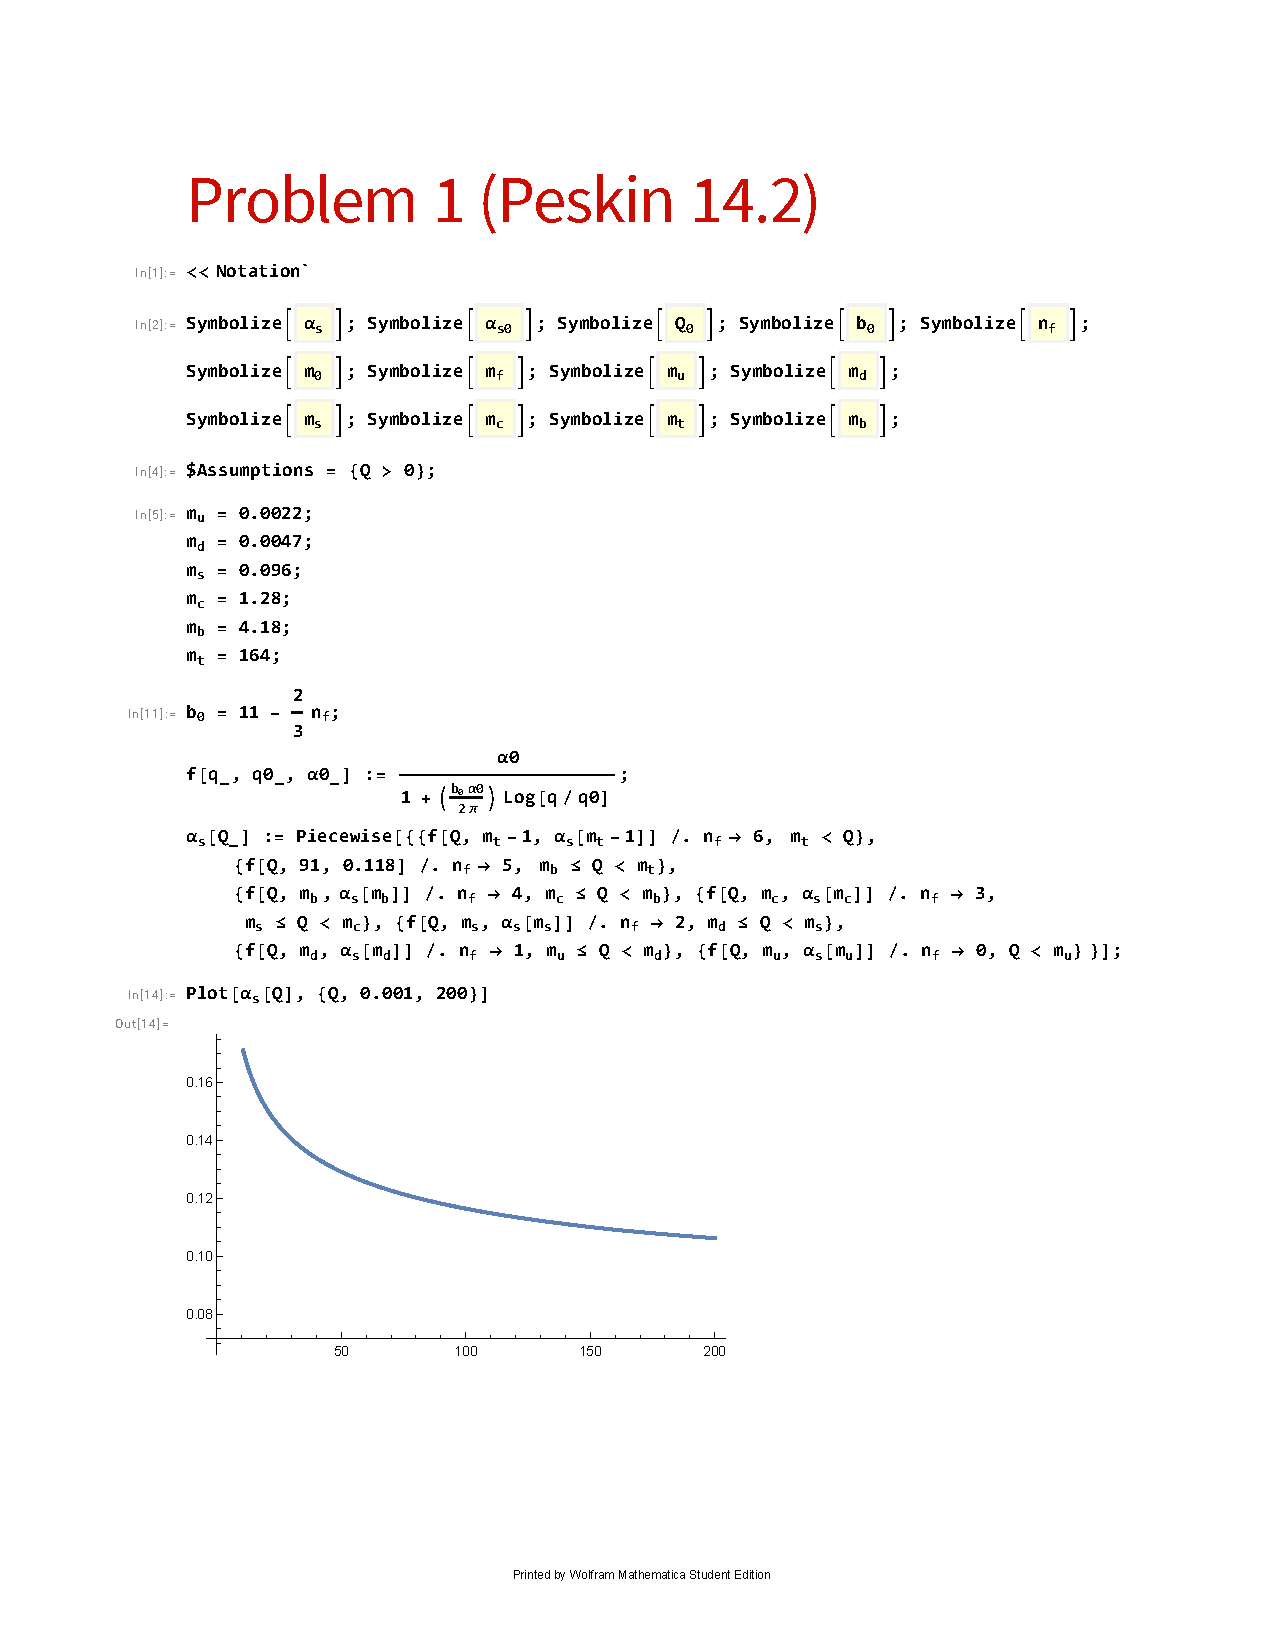
\includepdf[pages=-]{prob1.pdf}
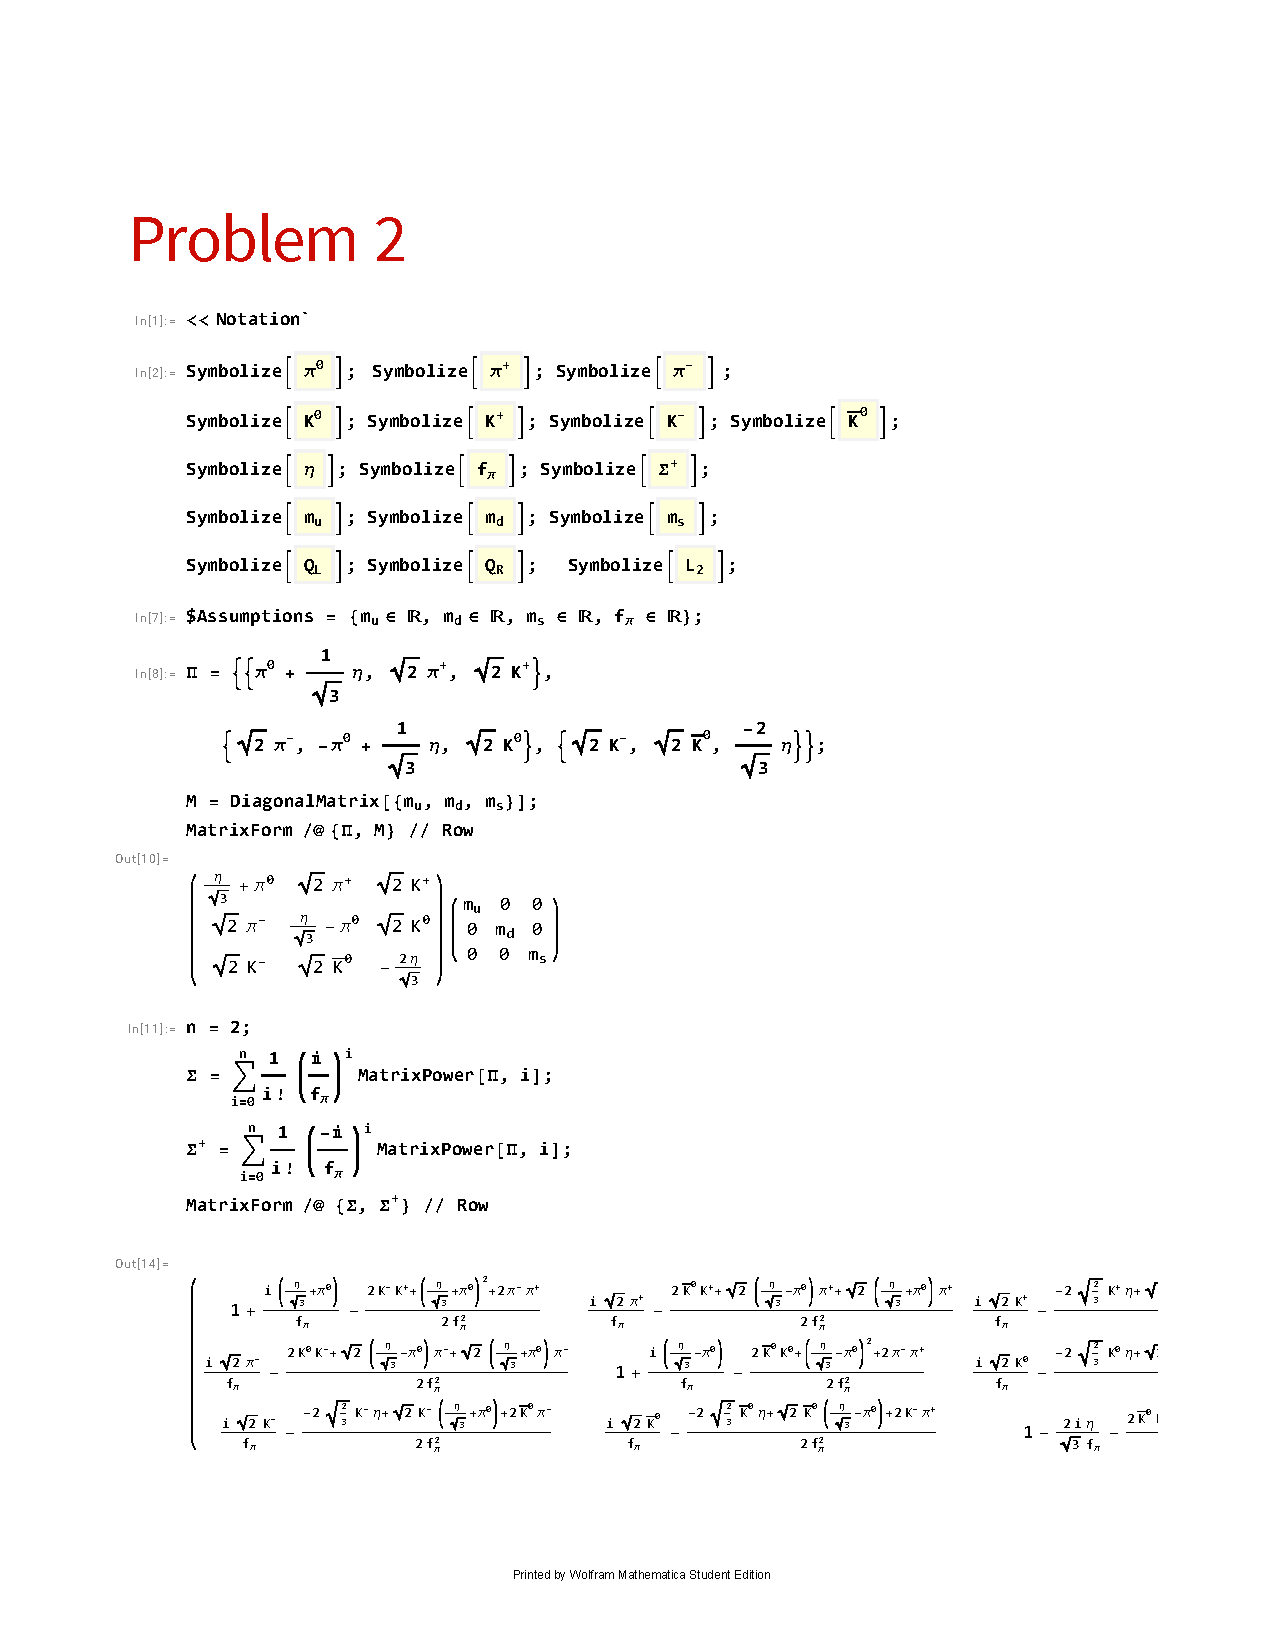
\includepdf[pages=-]{prob2.pdf}

\end{document}